\chapter{Knowledge Graph Visualization Tool}
Many existing knowledge graph visualizations are restricted to displaying certain types of relationships. 
Most commonly, a class hierarchy of an ontology is visualized for the user. Other graph visualization tools are capable of visualizing data.
 A few of these graph visualizers are mentioned in \nameref{chap:Related_work}.

What we didn't find is a graph visualizer capable of displaying complex class constructs, and a few features were missing as well.
Therefore, we decided to develop our own graph visualizer, which is capable of displaying class hierarchies with complex constructs.

This chapter will present the main features of our \textit{OWLVisualizer} and explain its capabilities and limitations.

\section{Main concept}
\label{sec:MainConceps}

We decided on 3 main components that the new framework should include:
\begin{itemize}
    \item Clear Visualization: Our first goal was to facilitate navigation through the knowledge graph by highlighting the relations and classes of the graph as clearly as possible. This could be achieved, for example, by using different colors for different classes or by highlighting a class and its associated classes to which a relation exists. Additionally, we aim to make the graph as clear as possible and reduce the number of nodes to those that are ultimately essential for visualization.
    \item To clarify the relations between the queries, we implement a query builder that, given a class, can point to other classes through the relation, which in turn can point to further classes through another relation, as long as the user desires or there are no further relations. This should be done without having to use the SPARQL query language, making it much easier for the user. The Query Builder outputs a filtered graph with the selected triples.
    \item Rule Based Inference: Since a part of our work relies on inferences, we want to implement an inference query that can indicate inferred parameters based on the input of certain classes. This use case is quite specific to our scenario, but it should also be able to map to other ontologies. The output should be an action tree with the inferred parameters and a visualized graph with the associated classes that play a role in the inference.
\end{itemize}

\section{Features}

\begin{figure}[H]
    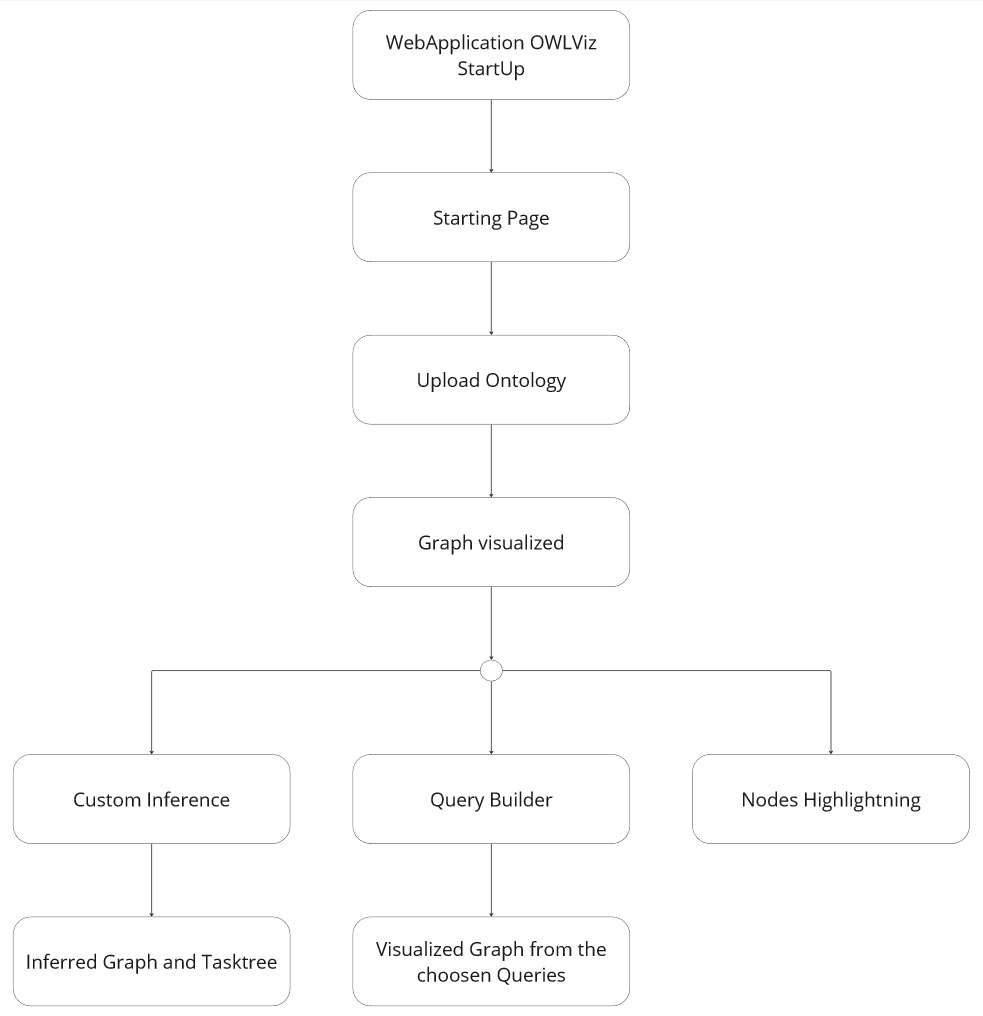
\includegraphics[scale=0.35]{Graphics/architecture_simplified.jpg}
    \label{fig:OWLViz_architecture}
    \caption{Architecture chart for the OWLVisualizer framework}
\end{figure}

\subsection{Graph Visualization}
In this section, we present a simple example of our framework, from processing the ontology to visualization in the web application. 
This is intended to facilitate the reader's understanding of our framework. 
For this purpose, we create a small and simple ontology to explain the program flow in a straightforward manner. 
Additionally, we aim to demonstrate how this ontology is processed and what the interface between the frontend and backend looks like.

The visualization library \cite{visjs} has been used to create graph visualization in web-browsers.

\begin{figure}[H]
    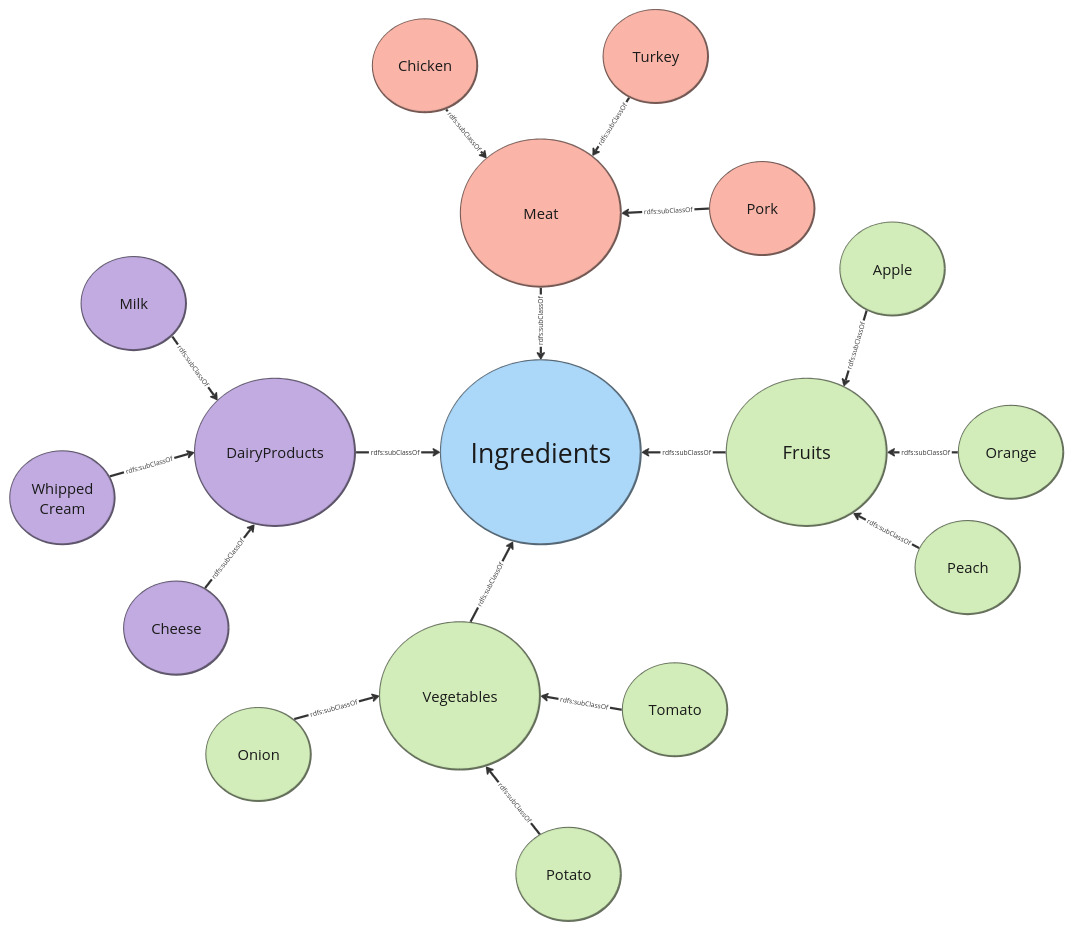
\includegraphics[scale=0.4]{Graphics/simple_ontology.jpg}
    \caption{Trivial example of an ontology}
\end{figure}
    
The ontology created for this purpose aims to provide a simple representation of various animal species. It includes superclass categories such as \textit{Fruits, Vegetables, Meat, and Dairy Products}, as well as subclasses like \textit{Apple} and \textit{Orange}, which are subclasses of the \textit{Fruits} superclass. This ontology does not depict complicated relations; rather, the individual classes are only connected to each other through the \textit{subClassOf} relation.

\subsection{Graph Processing}
The core component of the graph visualizer is the visualization of a hierarchy of classes. In this hierarchy, two nodes are connected by a directed edge, 
where the source node is the child node and the target node is the parent node. All edges are labeled either as \textit{subClassOf} or \textit{equivalentClass}.

To create the visualization from the graph, the ontology is parsed, and a triple matching process is applied to identify 
all classes that use \textit{subClassOf} or \textit{equivalentClass} as predicates.

By default, all nodes are uniformly colored green. However, in the \textit{mixing} and \textit{FoodCutting} ontologies, 
additional colors are used to highlight differences.
\begin{figure}[H]
    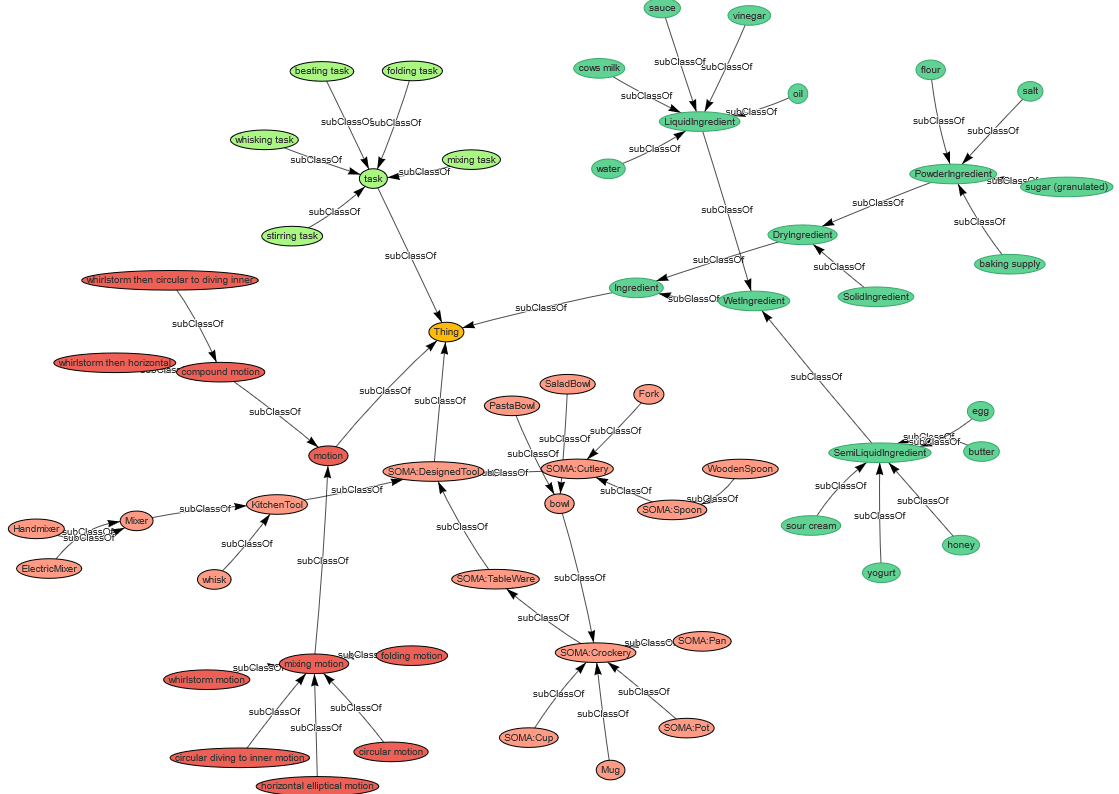
\includegraphics[scale=0.5]{Graphics/OwlVisualizer/graphProcessing1.png}
    \centering
    \caption{Processed Class Hierarchy}
\end{figure}

The graph visualizer is also capable of visualizing complex class expressions. 
However, it is essential to understand why the parsed expressions should not be used directly, as illustrated in figure \ref{fig:graphProcessing2}. 
Blank nodes and meta information associated with these expressions are generally useless to the user. 
This type of visualization is not compact, and users unfamiliar with ontology parsing will find it confusing and uninformative. 
Additionally, visualizing each parsed node increases the number of nodes and edges, which decreases performance of creating the graph visualization. 
Therefore, a more compact visualization of complex restrictions is necessary to ensure clarity and maintain optimal performance.

\begin{figure}[H]
    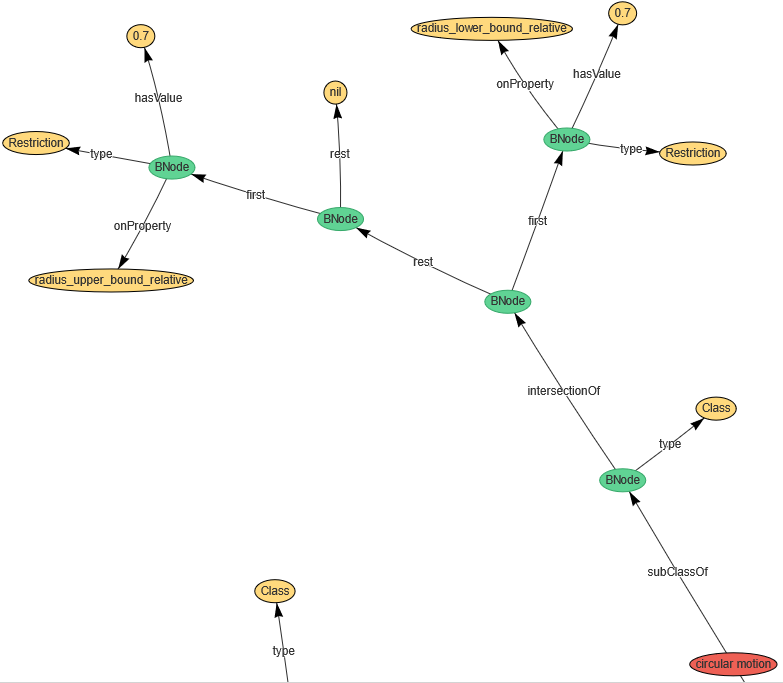
\includegraphics[scale=0.5]{Graphics/OwlVisualizer/graphProcessing2.png}
    \centering
    \caption{Visualize parsed class restrictions}
    \label{fig:graphProcessing2}
\end{figure}

To achieve a compact representation of class expressions, we recursively traverse the parsed class expression, 
searching for essential information such as the relations used and their corresponding values. 
All blank nodes are implicitly skipped and not visualized. Additionally, meta information is excluded.

The visualizer can also handle nested expressions, as well as intersections and unions. Each \textbf{AND} node indicates that all connected elements belong to the intersection.
Similarly, each \textbf{OR} node indicates that all connected elements belong to the union.

In the figure \ref{fig:graphProcessing3}, the following expression is visualized:

CircularMotion \textit{subClassOf} (radius upper bound relative value 0.7) and (radius lower bound relative value 0.7)

\begin{figure}[H]
    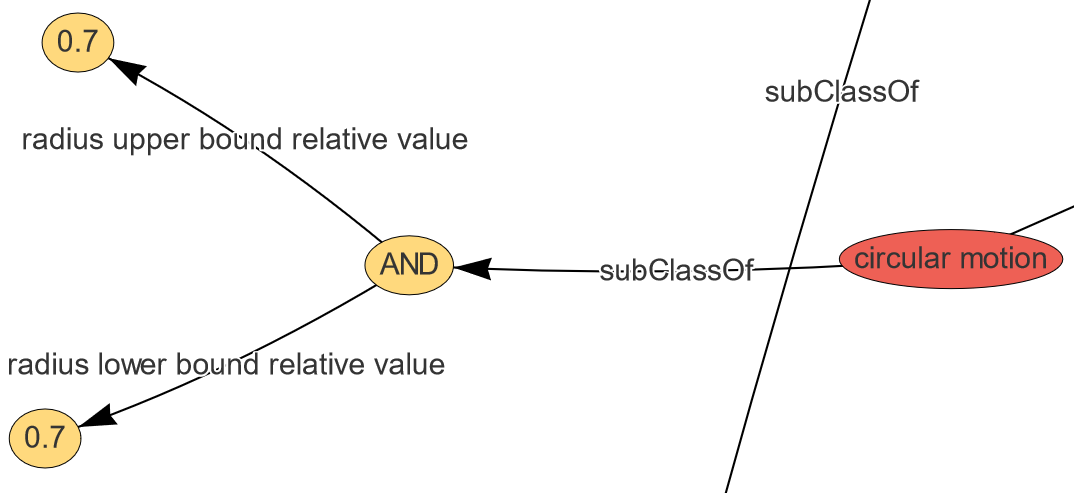
\includegraphics[scale=0.3]{Graphics/OwlVisualizer/graphProcessing3.png}
    \centering
    \caption{Compact representation of class expression}
    \label{fig:graphProcessing3}
\end{figure}

\subsection{Load Ontology}

By pressing the \textit{Load Ontology} button, users can load a wide range of ontologies that have the \textit{.owl} file extension.
Upon selecting the ontology, the \textit{OwlVisualizer} begins parsing the ontology to process the ontology. 
Once the processing is complete, a visual representation of the ontology is created, which can be explored by the users freely. 


\begin{figure}[H]
    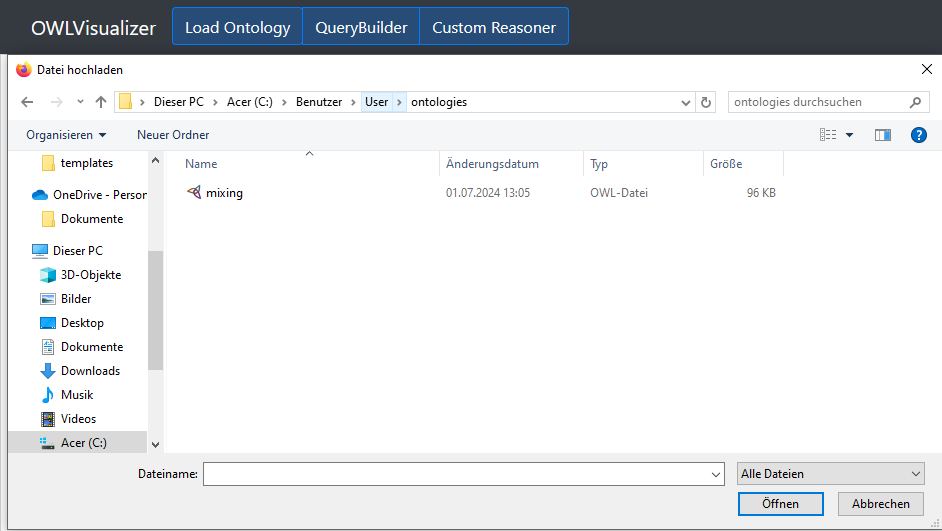
\includegraphics[scale=0.35]{Graphics/OwlVisualizer/loadOntology1.png}
    \centering
    \caption{Loading Ontology}
    \label{fig:loadOntology1}
\end{figure}

Attempting to load any other file types results in an error message being displayed on the website. 
When a user tries to upload a file that does not have the \textit{.owl} extension, the \textit{OWLVisualizer} notifies 
the user that the file extension is not supported by this tool, via an error message. 

\begin{figure}[H]
    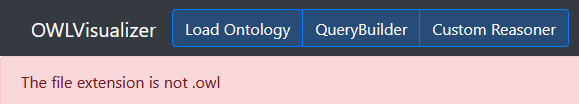
\includegraphics[scale=0.5]{Graphics/OwlVisualizer/loadOntology2.png}
    \centering
    \caption{\textbf{Error}: Unsupported File Type}
    \label{fig:loadOntology2}
\end{figure}

Additionally, if an ontology can't be parsed, an error message is thrown that ontology couldn't be
loaded properly. Whenever this issue is encountered during the parsing of the selected ontology, it immediately stops and triggers an error notification. 
This message informs the user that there was a problem with loading the ontology, possibly due to a formatting error or an unsupported structure within the file. 
This error message informs the user of this particular issue; the \textit{OWLVisualizer} doesn't attempt to deal with this problem.

\begin{figure}[H]
    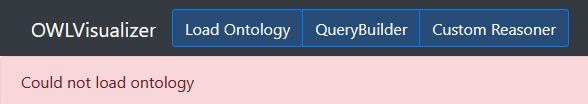
\includegraphics[scale=0.5]{Graphics/OwlVisualizer/loadOntology3.png}
    \centering
    \caption{\textbf{Error}: Ontology Load Failure}
    \label{fig:loadOntology3}
\end{figure}

\subsection{Search Classes}
The \textit{OwlVisualizer} includes a feature that suggests classes, which are visualized as nodes, 
for users to focus on, improving their ability to navigate and understand complex networks.

\begin{figure}[H]
    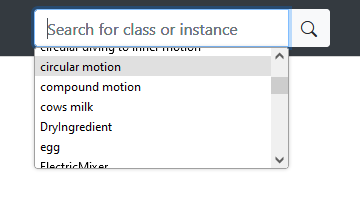
\includegraphics[scale=0.6]{Graphics/OwlVisualizer/searchClass1.png}
    \centering
    \caption{Search bar suggesting available classes}
\end{figure}

The key implementation for this feature is a search bar that suggests all visualized classes. 
Any nodes belonging to a class restriction are not suggested. 
The available suggestions are sorted in descending order, allowing users to easily search
for classes and explore the class hierarchy without assuming prior familiarity with the ontology.

\begin{figure}[H]
    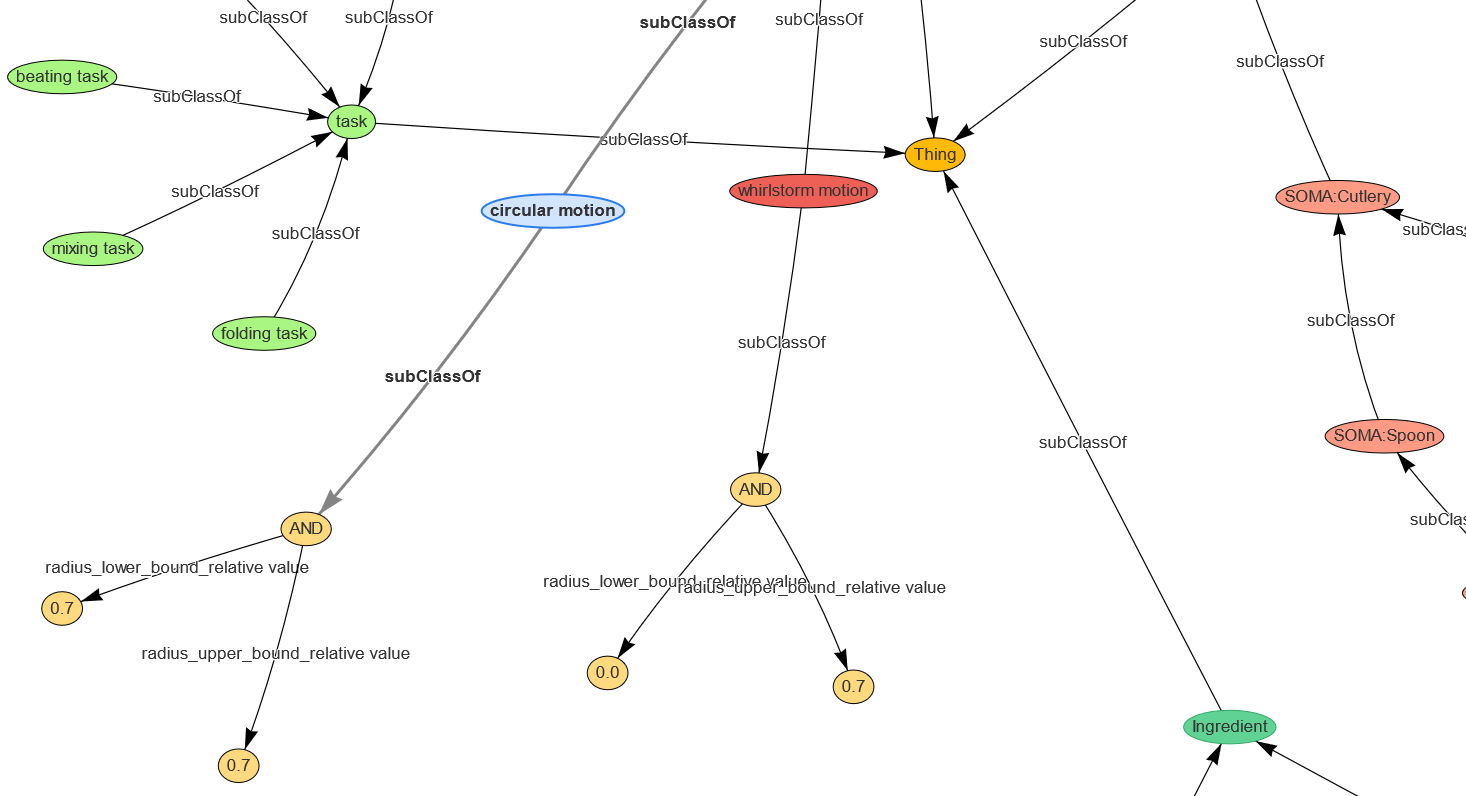
\includegraphics[scale=0.25]{Graphics/OwlVisualizer/searchClass2.png}
    \centering
    \caption{Focus node}
\end{figure}

Users can press Enter inside the search bar or click the search button to immediately focus on the chosen class. 
Focusing on the class is achieved by zooming to the respective node and highlighting it. 
This allows users to quickly identify the corresponding node along with all of its parent and child nodes.

\subsection{Custom Inference - Mixing}

One option for the user to execute functions on a graph is the Inference Builder. 
It's important to note that the Custom Inference Builder is not a generic use case and in this version, it's tailored to the Mixing Graph (see \nameref{chap:Data_representation}). 
In our case, we infer a motion and its corresponding parameters based on a given task and a list of ingredients. 
\begin{figure}[H]
    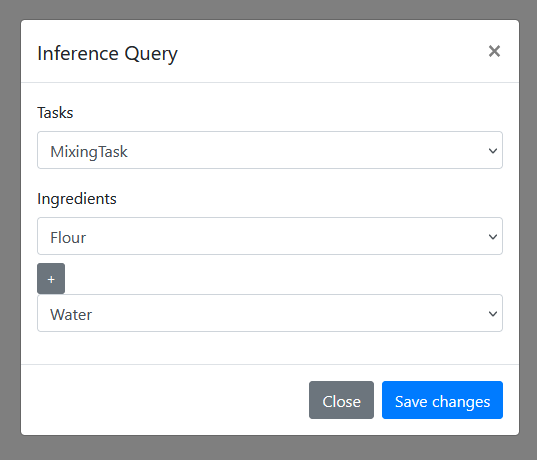
\includegraphics[scale=0.45]{Graphics/inference_user_input.png}
    \caption{Select fields for the inference.}
\end{figure}
The Custom Inference Builder then generates a graph that only displays the corresponding nodes for clarity, as well as a task tree that can be followed by an agent.
In the first step, the task and the ingredients are sent to the backend for inference, which in turn sends back the inferred motion and parameters to the frontend.
The backend function processes the inference with the received parameters, which results in a task tree as well as a filtered graph, that contains only the classes that are used in the inference, these are then used for visualization.
In the frontend, the data is processed using an \textit{AJAX} request. After sending the task and the list of ingredients, the response, which includes the generated graph and task tree, is returned to the frontend and processed. A \textit{JavaScript}-function then creates a graph with the nodes and edges received from the backend and generates a table with a variable number of rows based on the backend's output.
After processing the data, the graph and the task tree are visualized based on the user input.

\begin{figure}[H]
    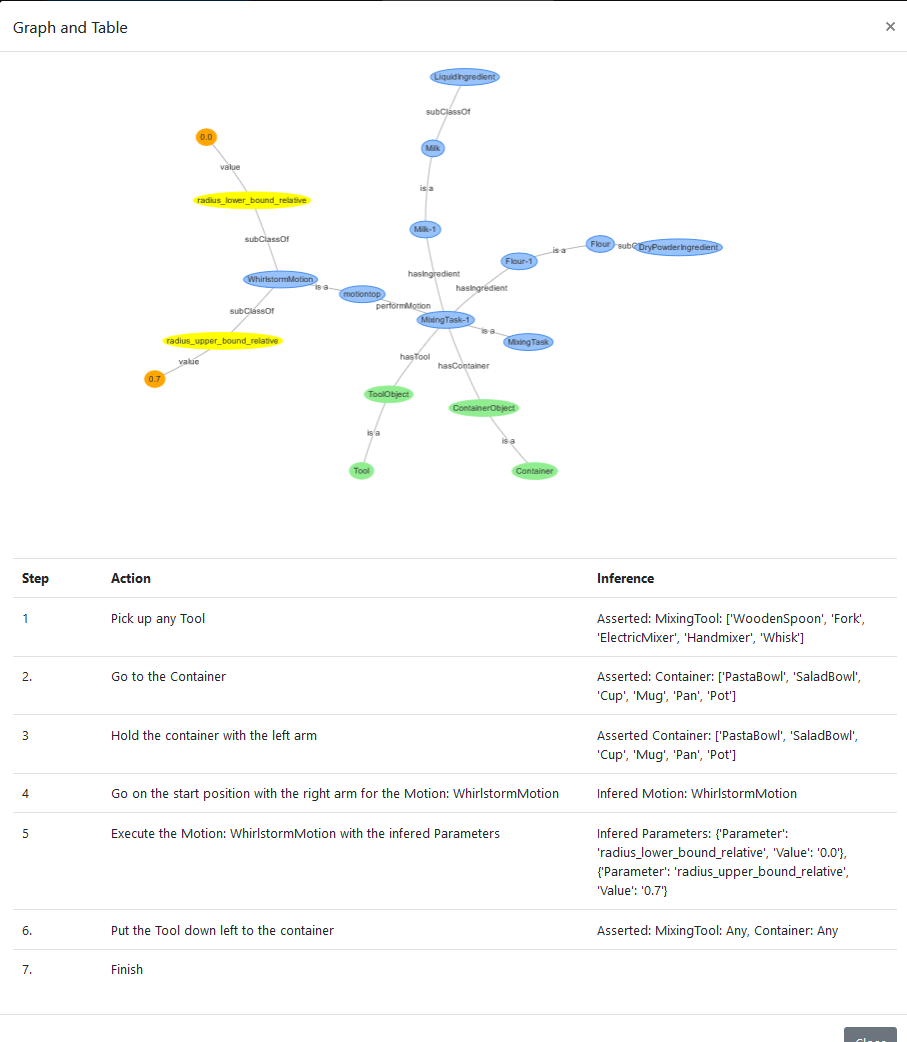
\includegraphics[scale=0.5]{Graphics/new_inference_graph.png}
    \caption{inferred graph and task tree.}
    \label{fig:graph_inferred}
\end{figure}

The data processing and the detailed implementation of the Inference Builder will be further explained in the \nameref{sec:Implementation} section.
\subsection{QueryBuilder}
The QueryBuilder is a feature that provides users with suggested triples, allowing them to explore the graph in an intuitive manner.
No SPARQL knowledge is required. This feature generates a visualization of the selected triples and constructs a SPARQL query, 
which only needs slight modification to be queryable.

\paragraph{Triple Matching}
Triple Matching allows users to select a subject, predicate, and object to explore the graph. 
At the beginning of the triple matching process, all classes are available as subjects. 

\begin{figure}[H]
    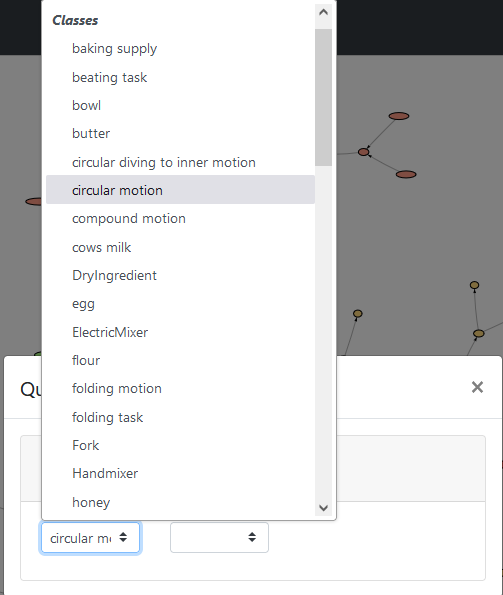
\includegraphics[scale=0.4]{Graphics/OwlVisualizer/queryBuilder1.png}
    \centering
    \caption{Focus node}
\end{figure}

Only predicates that appear as edge labels connected to the subject in the graph are suggested. 

\begin{figure}[H]
    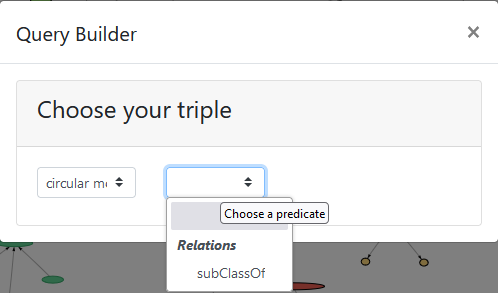
\includegraphics[scale=0.4]{Graphics/OwlVisualizer/queryBuilder2.png}
    \centering
    \caption{Focus node}
\end{figure}
Similarly, only objects connected to the subject via the selected edge are proposed. 

\begin{figure}[H]
    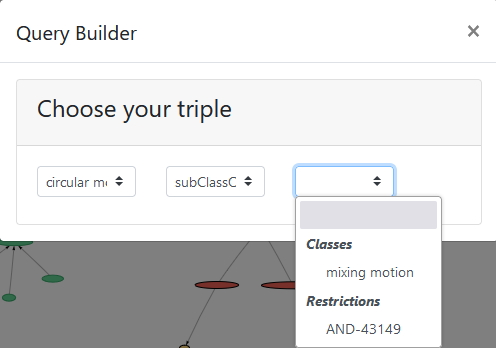
\includegraphics[scale=0.4]{Graphics/OwlVisualizer/queryBuilder3.png}
    \centering
    \caption{Focus node}
\end{figure}
Once a triple is selected, the user can continue to explore the graph based on the previously chosen triples.

All complex class expressions are processed in a single triple matching step, whereas navigating through the class hierarchy occurs incrementally.

Whenever a triple is selected, the QueryBuilder creates a tab with two items, one item visualizes the graph, the other item 
contains a SPARQL query. 
\paragraph{View Graph}
In the View Graph, users can inspect the graph based on their selection of triples. 
This view is a subgraph, which makes it easier to inspect the relationships between classes and classes with complex class expressions. 
Each class expression is displayed in a separate view, allowing users to focus on each class expression independently, which also reduces clutter in the graph. 
The class hierarchy has its own view, which can be incrementally updated with new classes to view hierarchical relationships. 
Separating the views ensures that users can navigate and explore different aspects of the graph, while also improving their comprehension of the ontology.

\begin{figure}[H]
    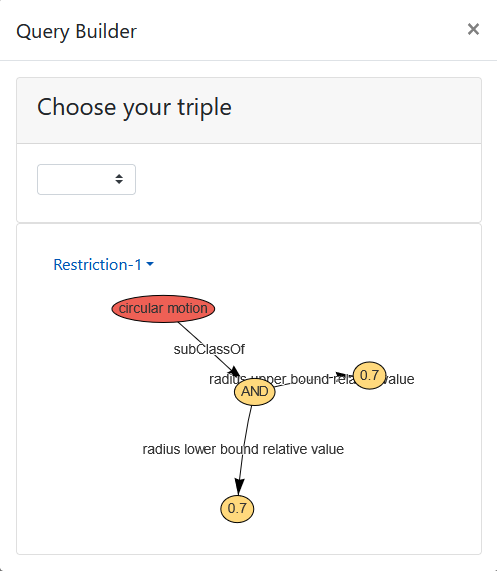
\includegraphics[scale=0.4]{Graphics/OwlVisualizer/queryBuilder4.png}
    \centering
    \caption{Focus node}
\end{figure}

\paragraph{SPARQL Query}
A SPARQL ASK query is generated for each chosen triple. If the triple is querying the hierarchy, the SPARQL query for querying the hierarchy is updated with the newest triples.
For each complex class expression, a separate query corresponds to the view of the subgraph.

This query is a queryable triple pattern that asks if this query pattern has a solution or not. 
Users can then independently modify and adapt this pattern to suit their specific needs. 
This feature will help users unfamiliar with querying ontologies by providing them with the triple pattern.
\begin{figure}[H]
    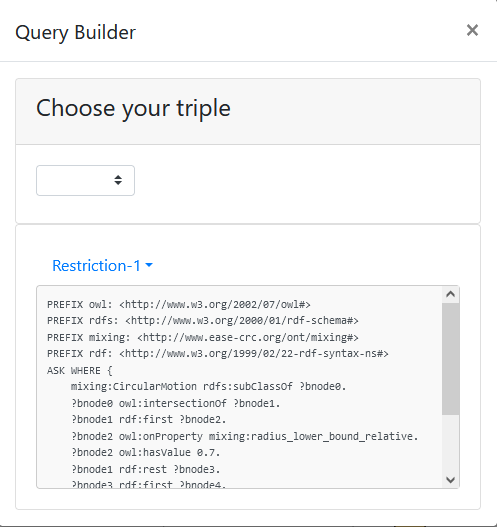
\includegraphics[width=0.5\textwidth]{Graphics/OwlVisualizer/queryBuilder5.png}
    \centering
    \caption{Focus node}
\end{figure}

\section{Limiations}

\paragraph{Using vis.js}
Using the graph visualization library vis.js yields poor performance on large graphs.
This reason is known to the developers of vis.js (See reference) and the cause of the problem is coming
from the physics simulation. The visualized graph is a force directed graph and the physics simulation attempts to make a user readable graph 
by seperating and clustering nodes who don't or belong to each other. This is done iteratively and consumes a lot of time for large sets of nodes
connected via many edges. The more interconnected the graph is the more terrible the performance gets. 

\paragraph{Data Visualizer}
This framework in its core is not a graph data visualizer. While it is absolutely able to display relationships and attributes of instance data, visualizing 
large datasets defined as ontology is not feasible. It is limited by vis.js which is poorly optimised for large sets of nodes and edges. 
Thus this framework can't be a graph data visualizer. 